\chapter{Main questionnaire form}
\label{app:questionnaire_form}
This appendix will include the questionnaire form I used to collect data from my main sample. This questionnaire is written in Norwegian and can be viewed starting from the next page. 
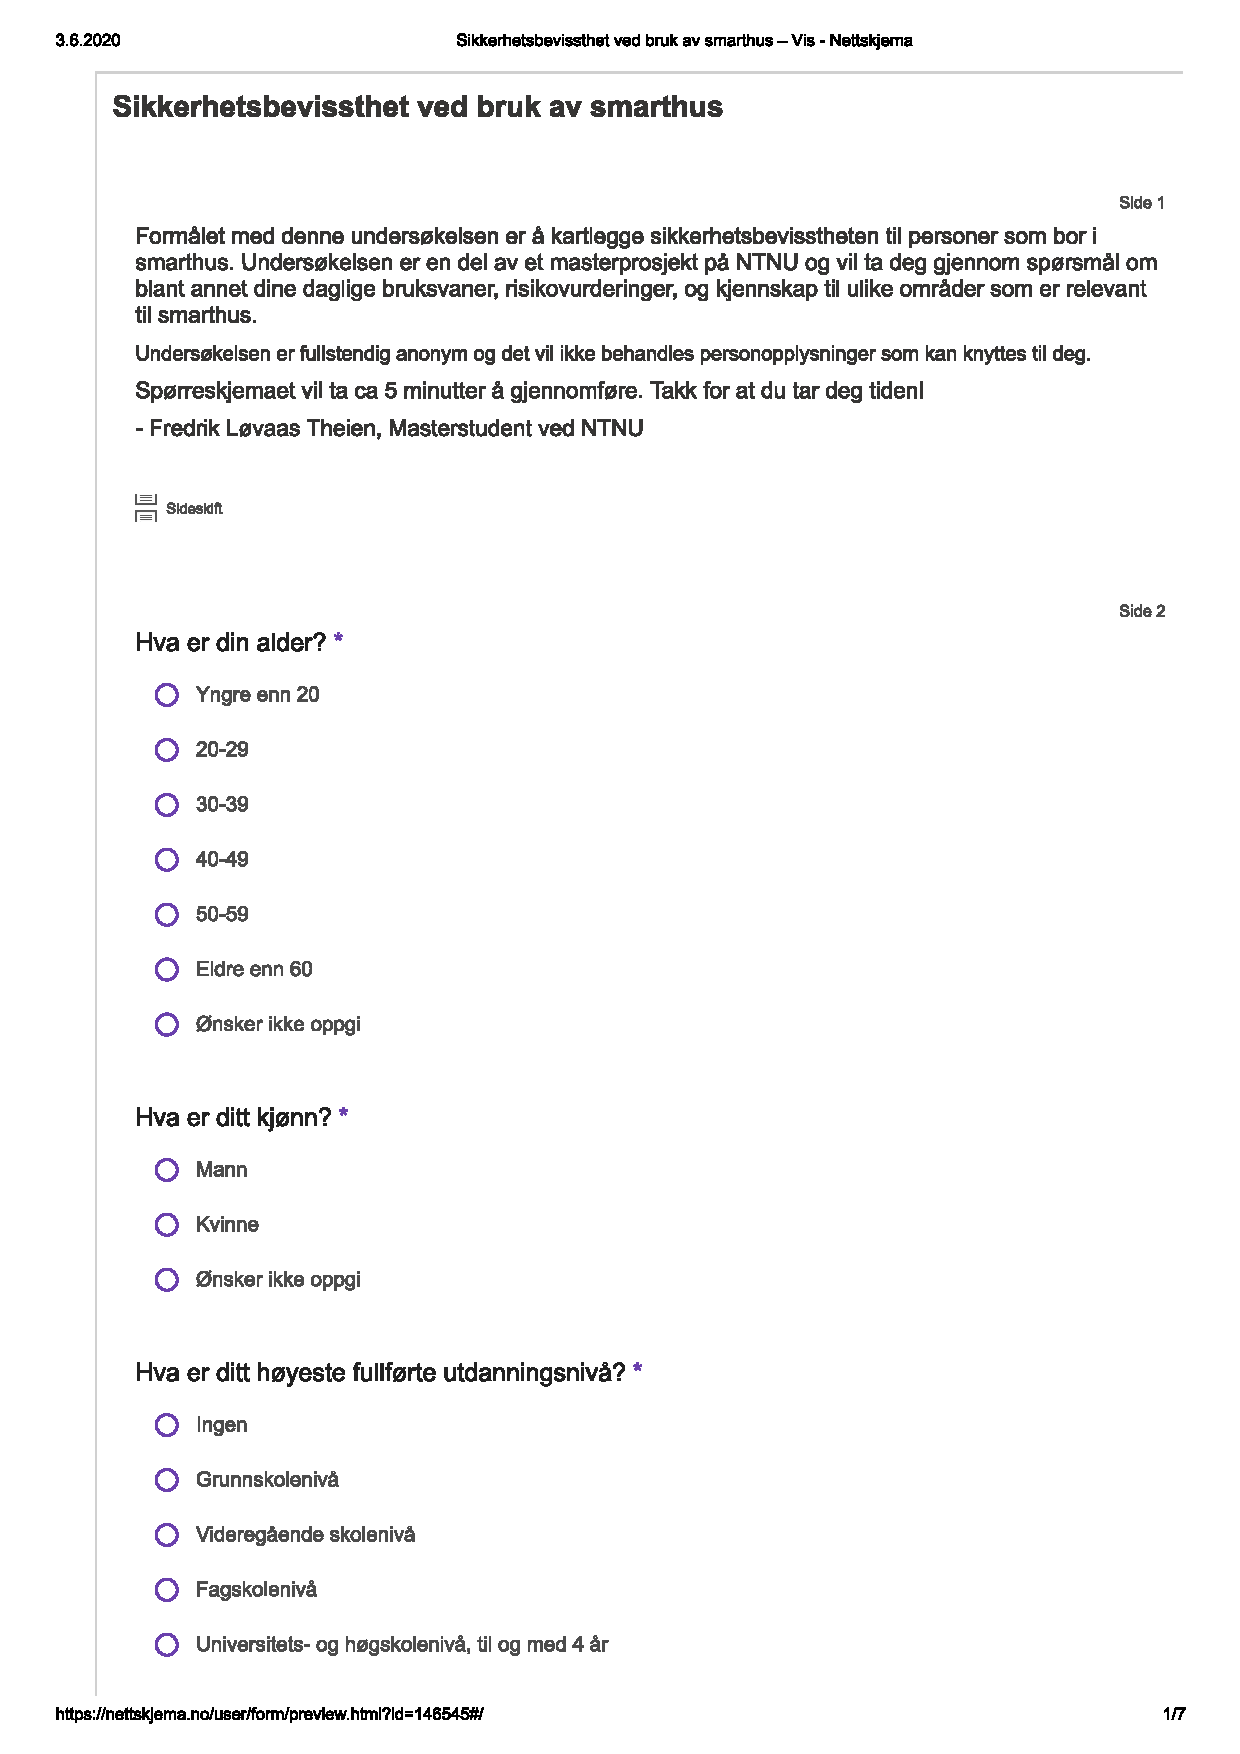
\includepdf[pages=-]{figures/pdfs/questionnaire.pdf}

\chapter{Control group questionnaire form}
\label{app:controlgroup_questionnaire_form}
This appendix will include the questionnaire form I used to collect data from my control group sample. This questionnaire is written in Norwegian and can be viewed starting from the next page.
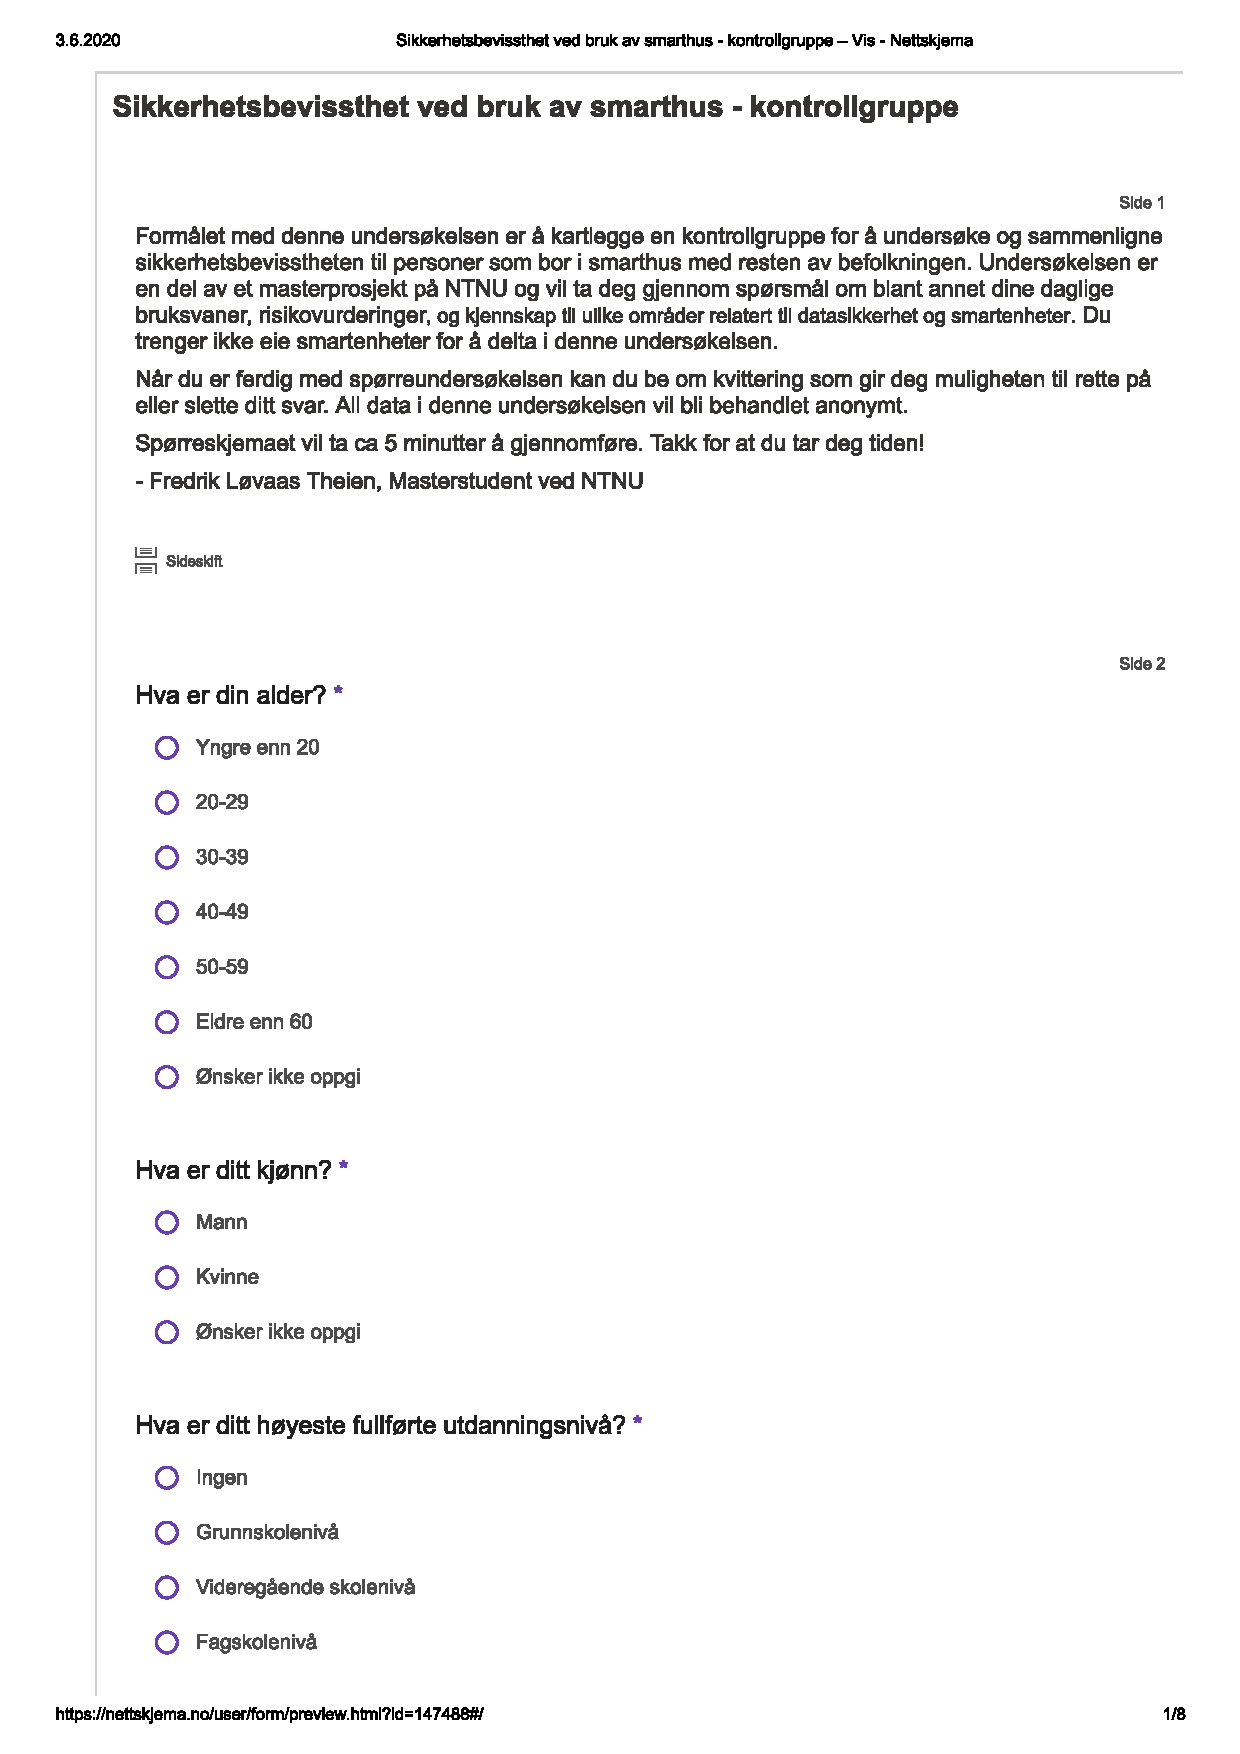
\includepdf[pages=-]{figures/pdfs/questionnaire-control-group.pdf}

\chapter{Bivariate analysis of age differences}

\begin{figure}[!h]
    \centering
    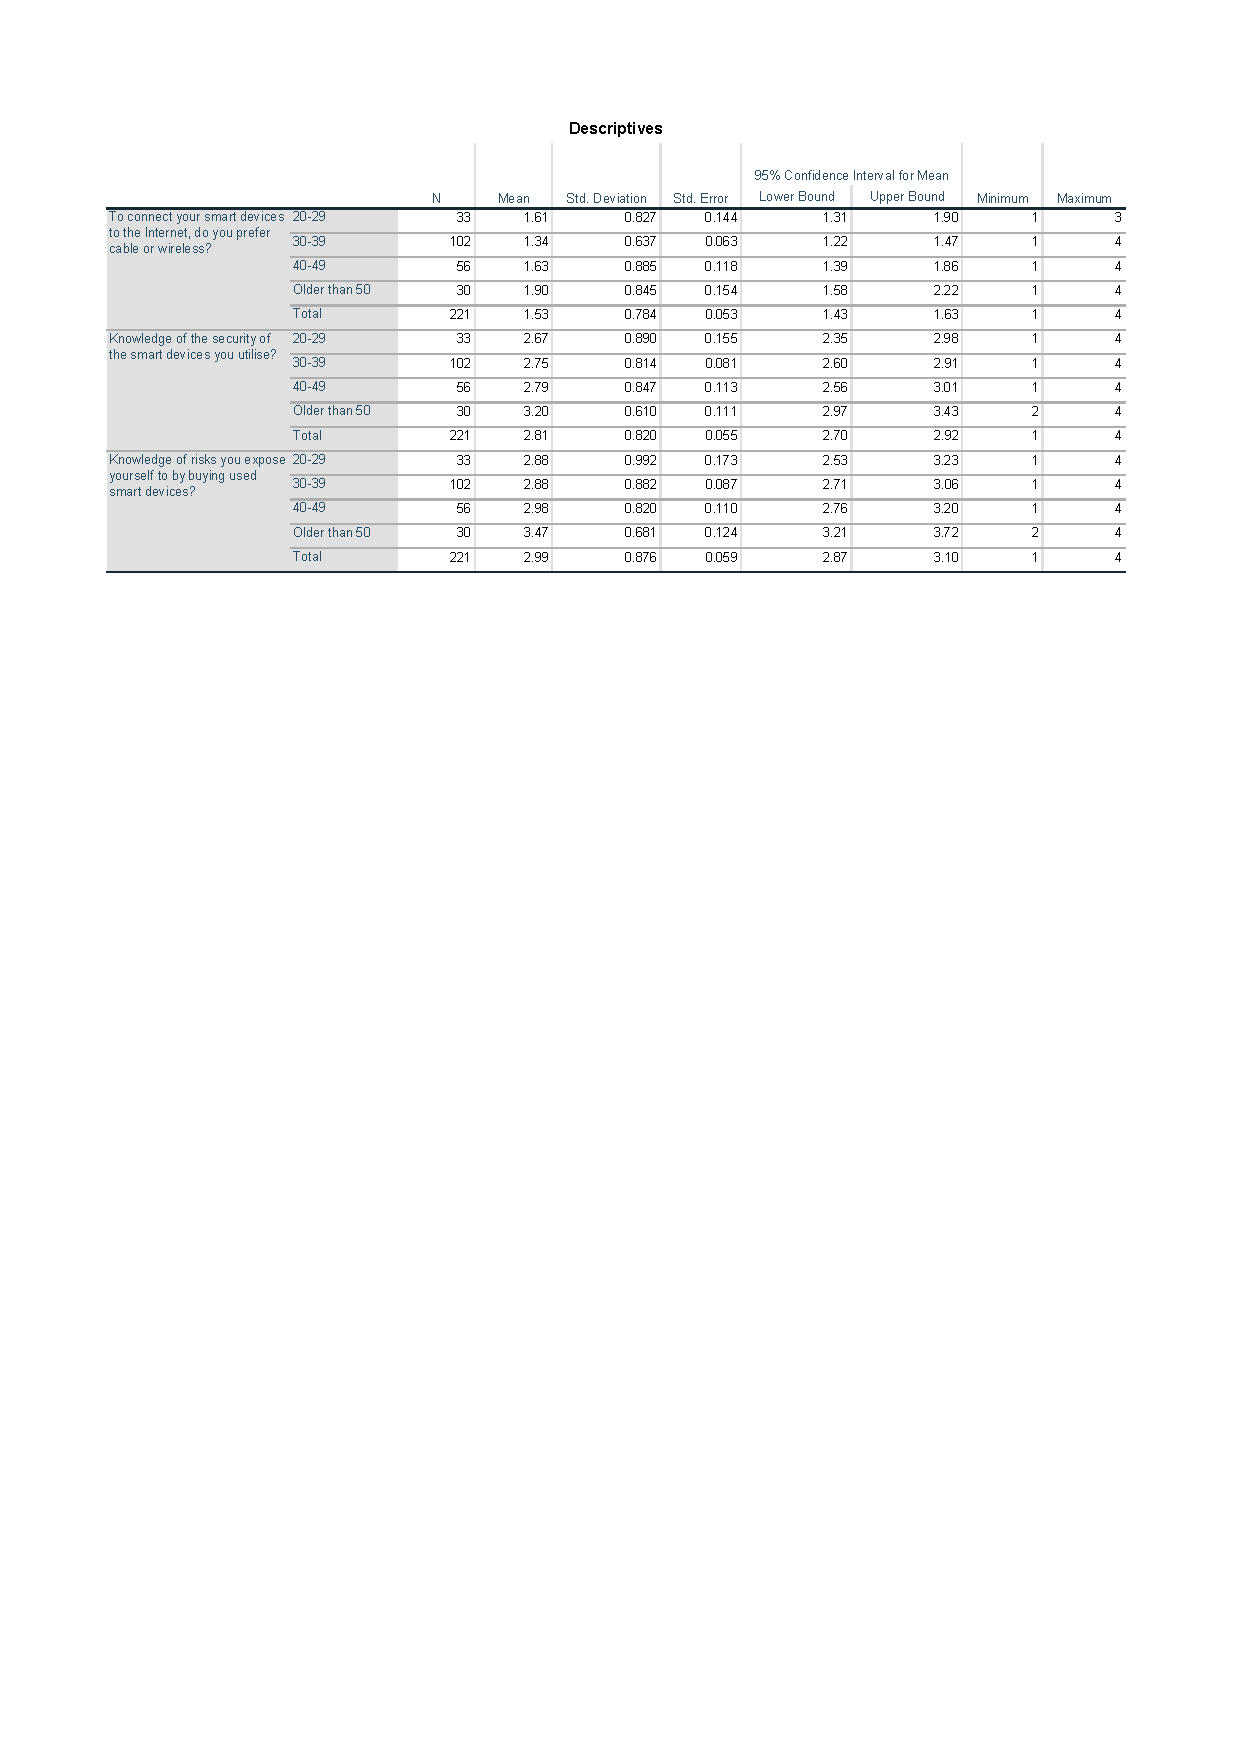
\includegraphics[scale=0.7]{figures/tables/anova_age_desc.pdf}
    \caption{Descriptive statistics of age up against other variables}
    \label{fig:anova_age_desc}
\end{figure}

\begin{figure}[!h]
    \centering
    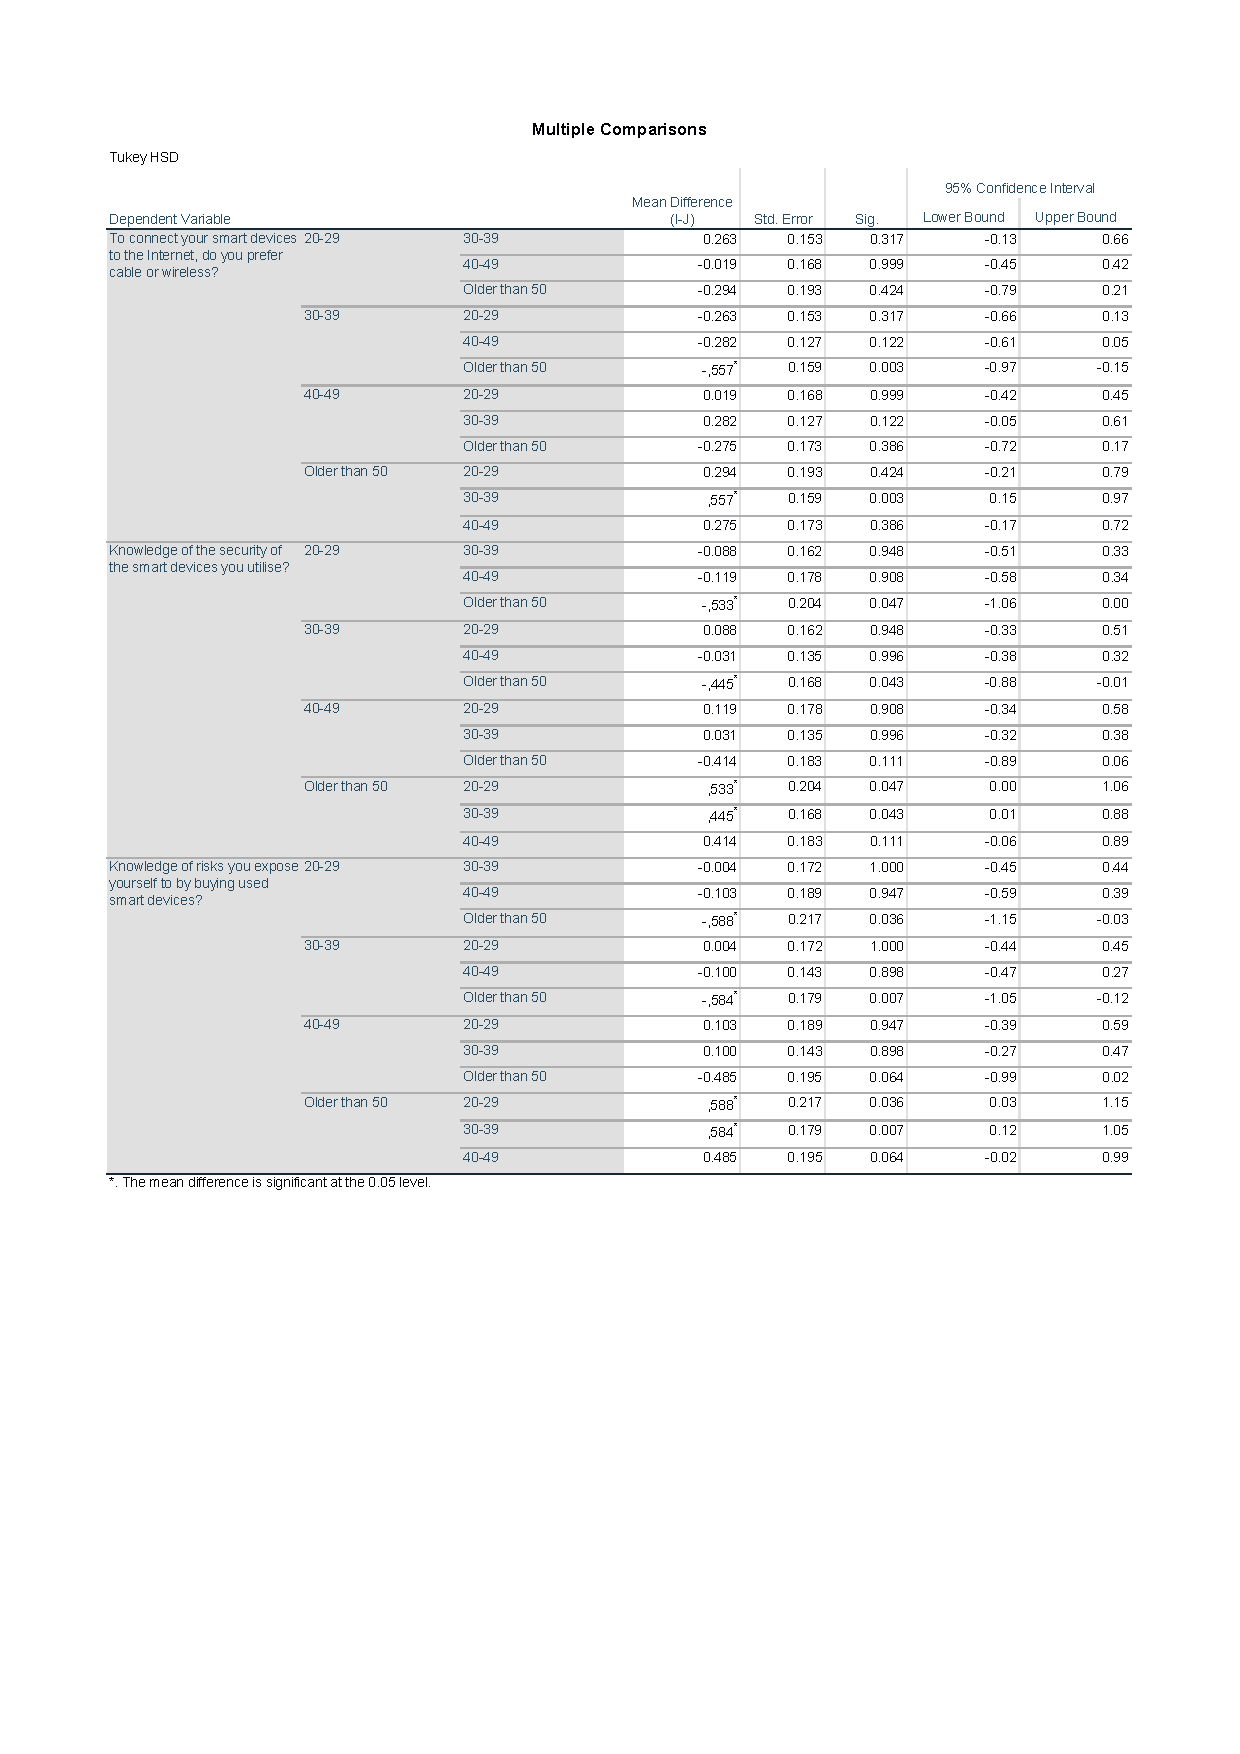
\includegraphics[scale=0.7]{figures/tables/anova_age_tukey.pdf}
    \caption{Post-hoc tukey of age categories up against other variables}
    \label{fig:anova_age_tukey}
\end{figure}

\chapter{Bivariate analysis of education differences}

\begin{figure}[!h]
    \centering
    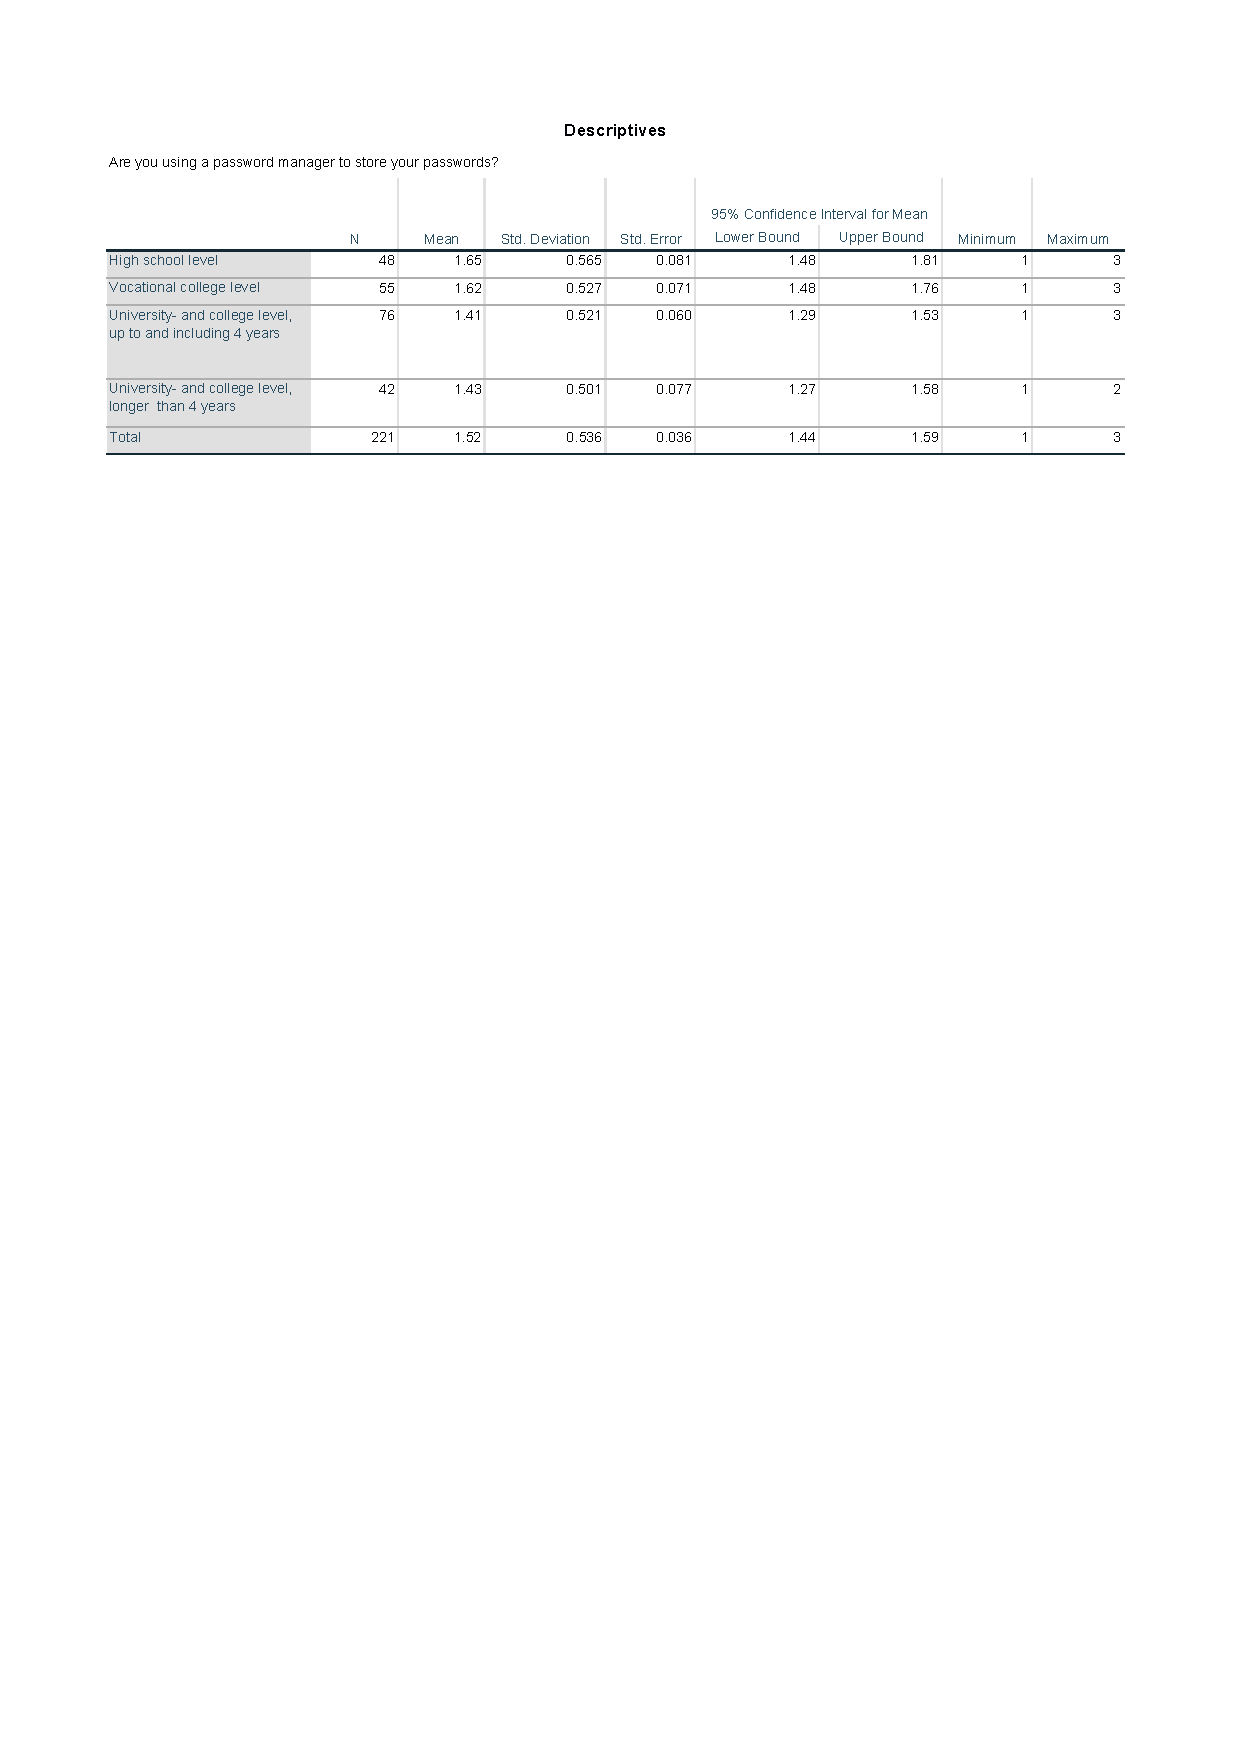
\includegraphics[scale=0.7]{figures/tables/anova_education_desc.pdf}
    \caption{Descriptive statistics of education up against the use of password managers}
    \label{fig:anova_education_desc}
\end{figure}

\begin{figure}[!h]
    \centering
    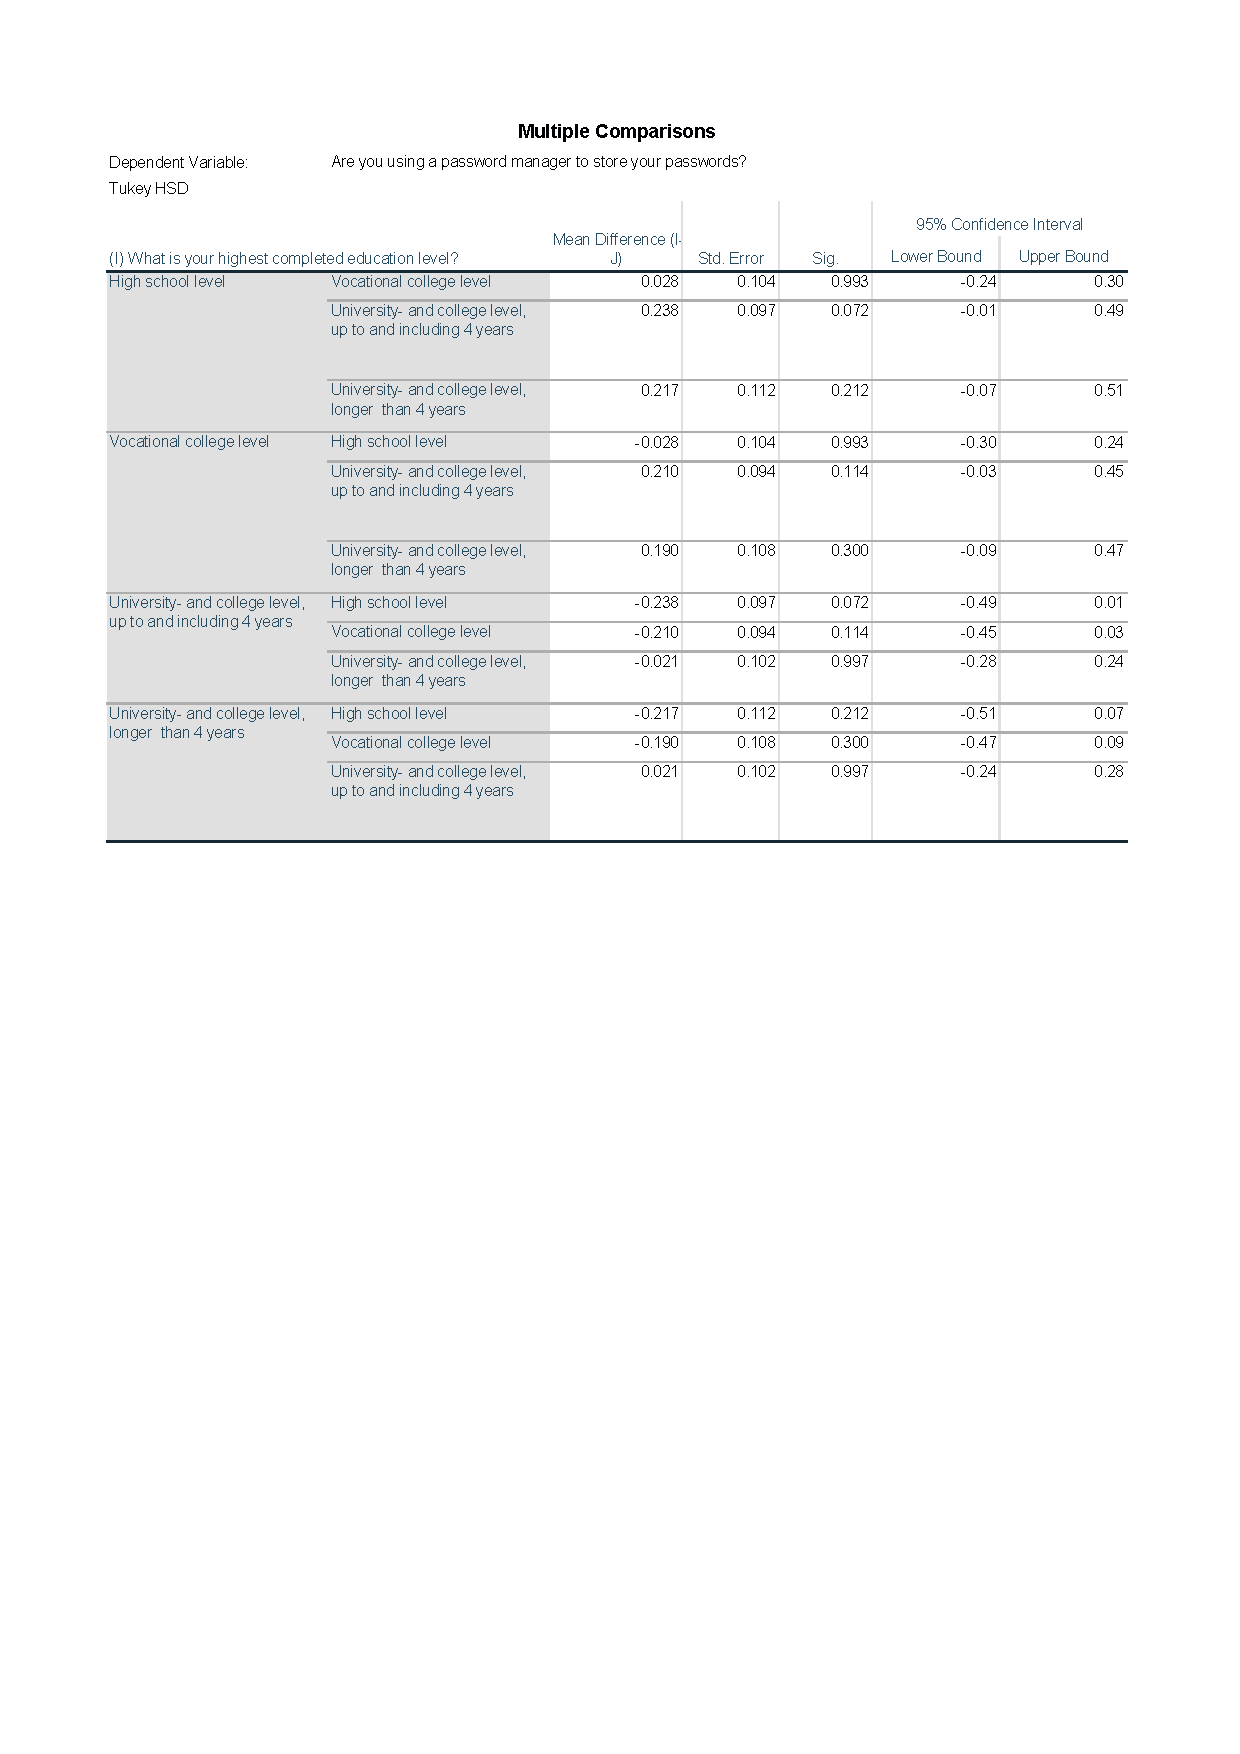
\includegraphics[scale=0.7]{figures/tables/anova_education_tukey.pdf}
    \caption{Post-hoc tukey of education categories up against the use of password managers}
    \label{fig:anova_education_tukey}
\end{figure}

\chapter{Analysis of changing settings and knowing data flow}

\begin{figure}[!h]
    \centering
    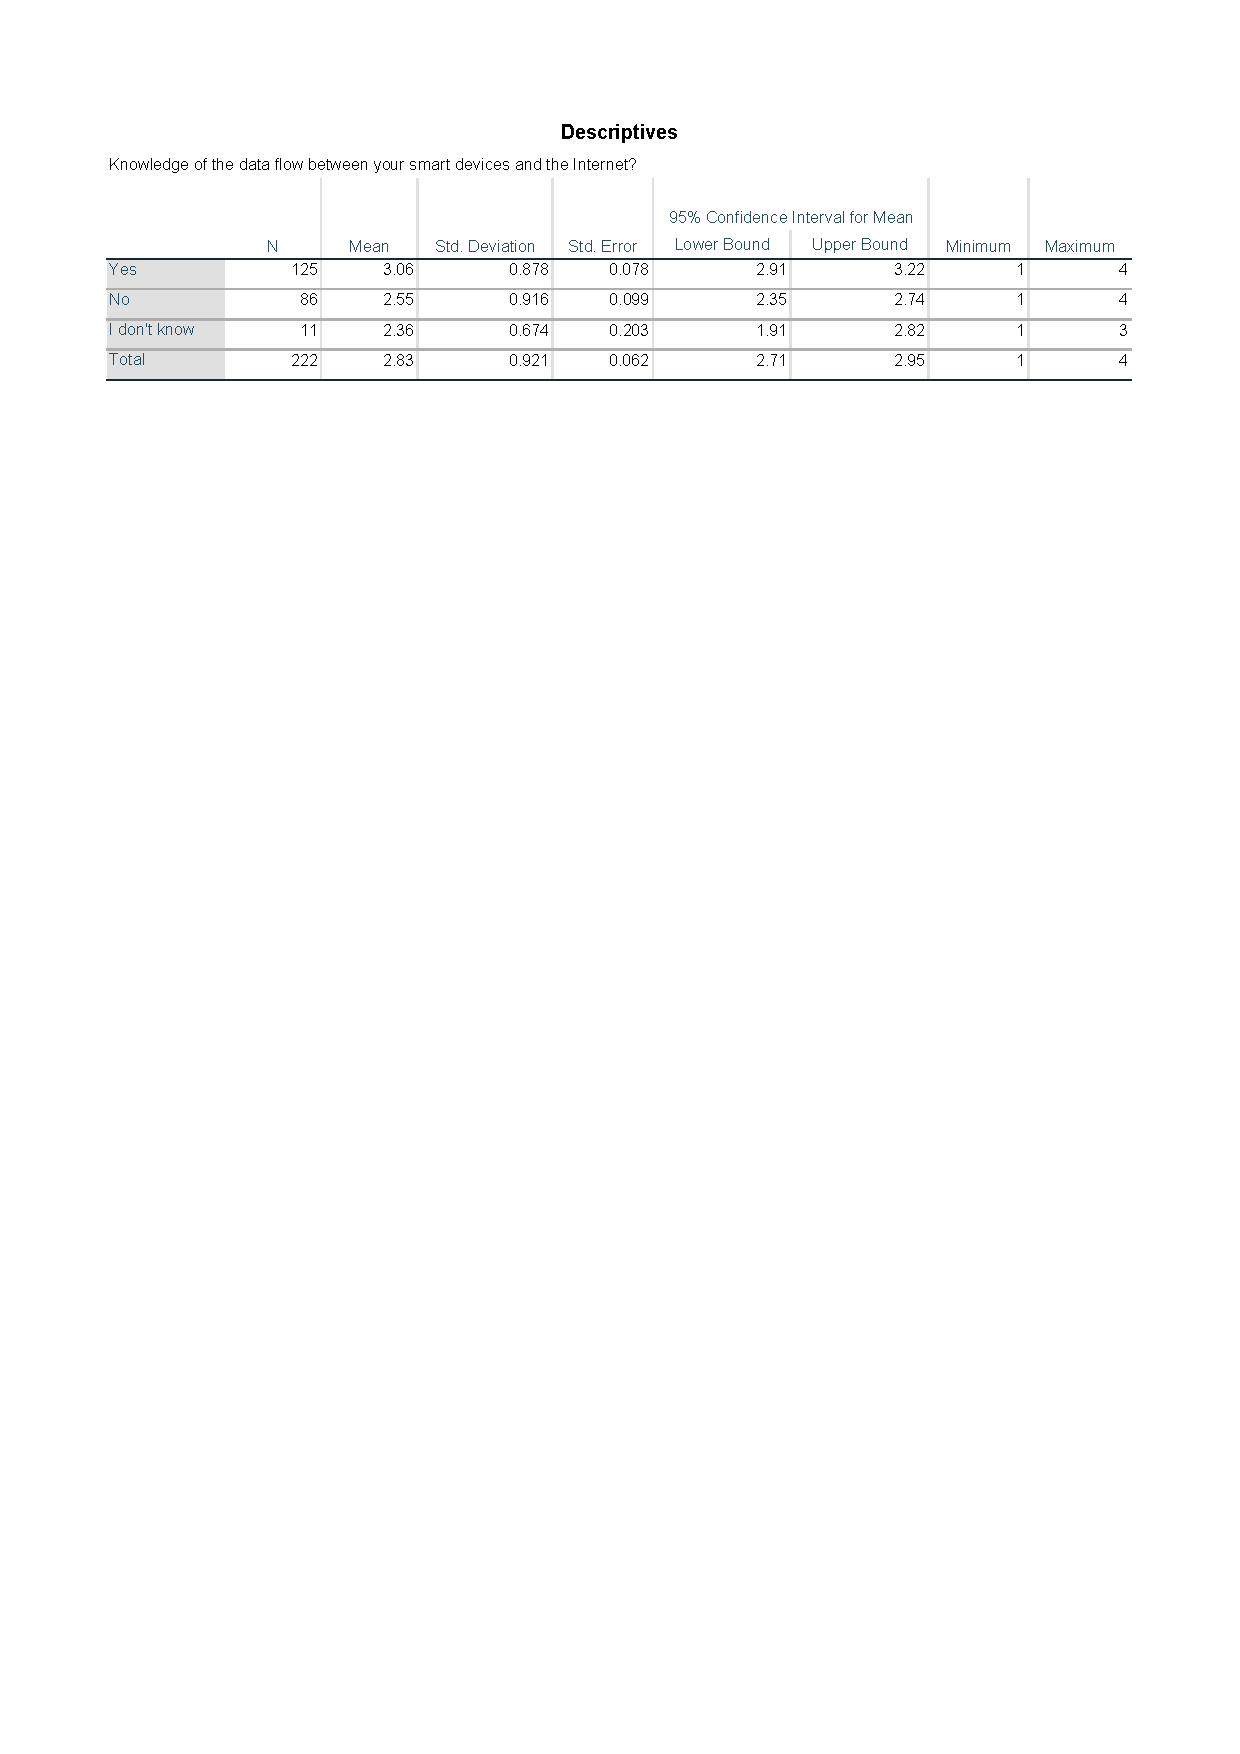
\includegraphics[scale=0.7]{figures/tables/anova_changesettings_dataflow_desc.pdf}
    \caption{Descriptive statistics of changing privacy and security settings and knowledge of data flow}
    \label{fig:anova_changesettings_dataflow_desc}
\end{figure}

\begin{figure}[!h]
    \centering
    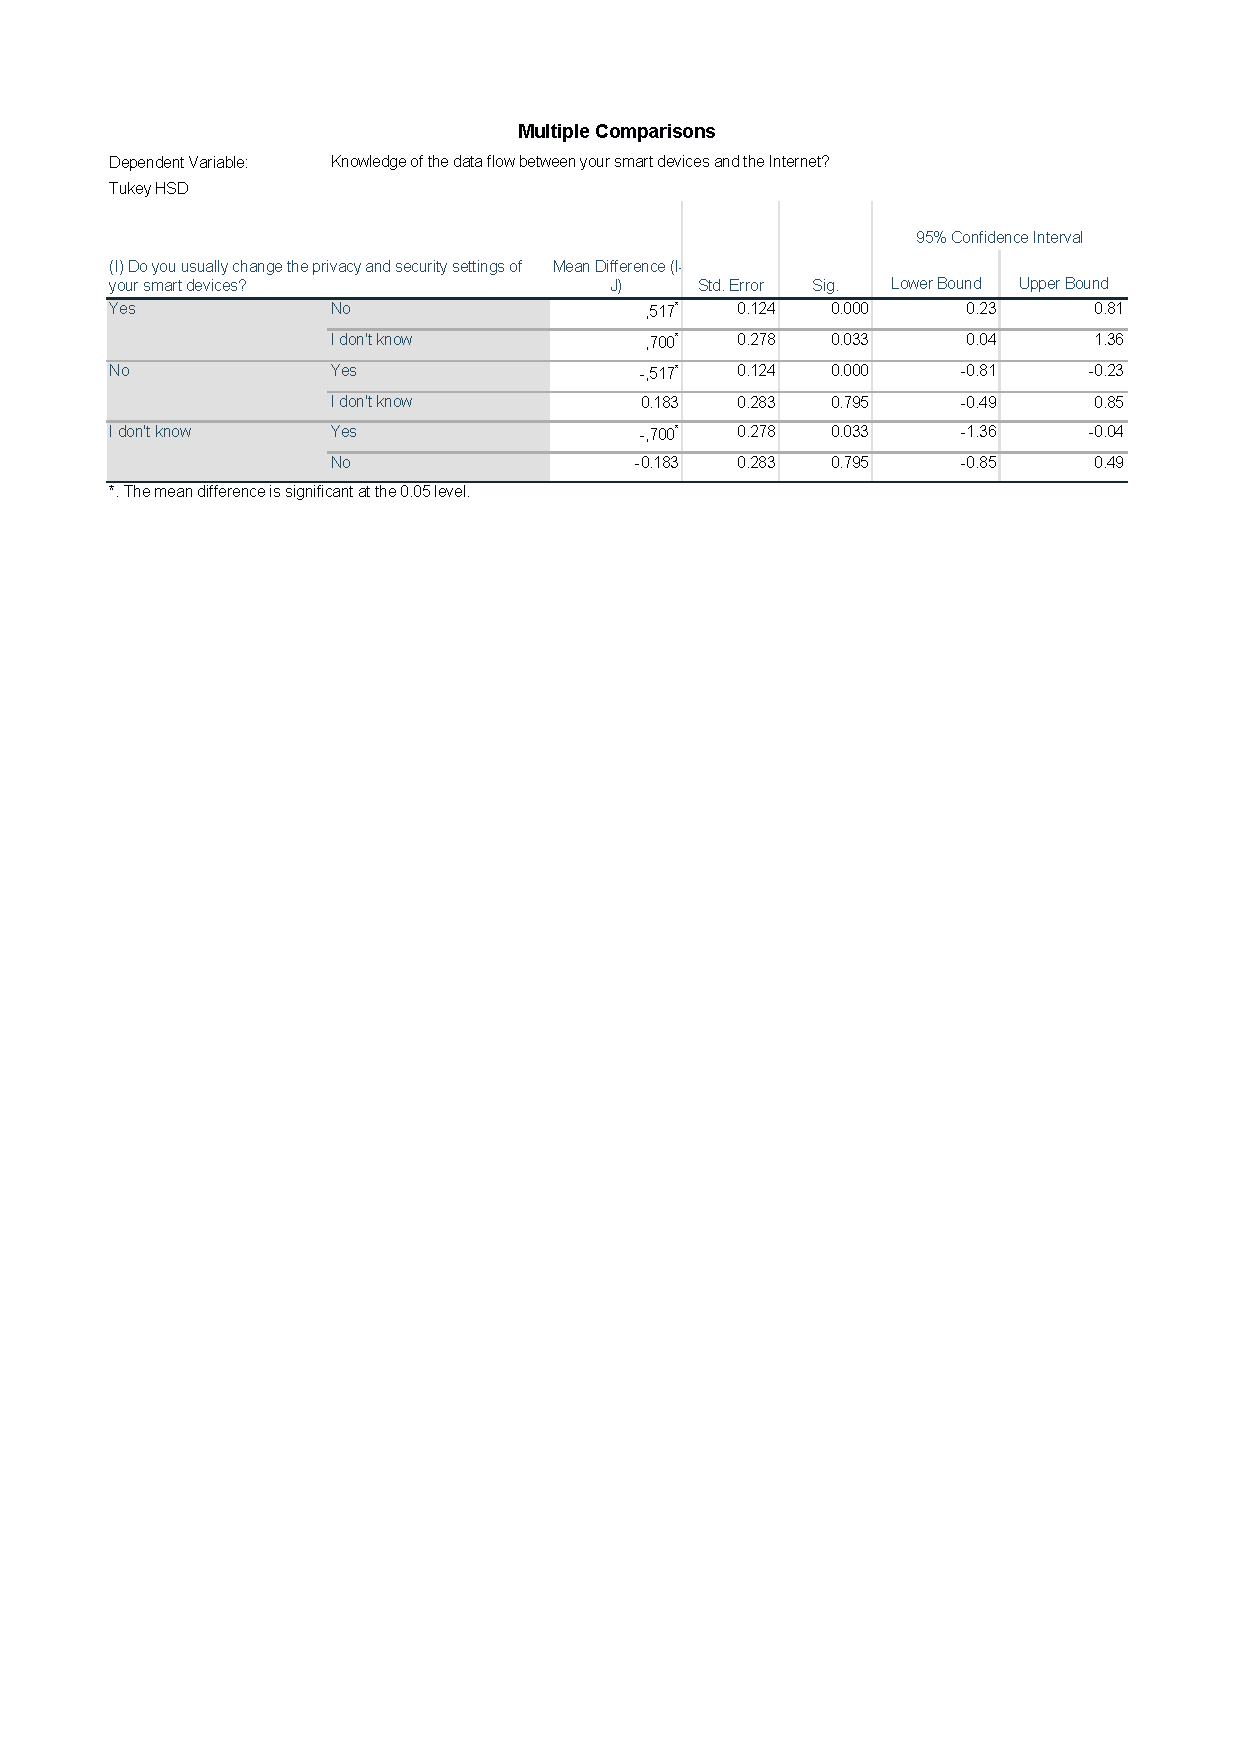
\includegraphics[scale=0.7]{figures/tables/anova_changesettings_dataflow_tukey.pdf}
    \caption{Post-hoc tukey of changing privacy and security settings and knowledge of data flow}
    \label{fig:anova_changesettings_dataflow_tukey}
\end{figure}

\chapter{Analysis of differences between the control group and main sample}
\begin{table}[!h]
\centering
\begin{tabular}{|l|r|r|r|r|r|}
\hline
\multicolumn{6}{|c|}{{\color[HTML]{010205} \textbf{Descriptive Statistics of Perceived Risk}}} \\ \hline
{\color[HTML]{264A60} } &
  \multicolumn{1}{c|}{{\color[HTML]{264A60} N}} &
  \multicolumn{1}{c|}{{\color[HTML]{264A60} Min}} &
  \multicolumn{1}{c|}{{\color[HTML]{264A60} Max}} &
  \multicolumn{1}{c|}{{\color[HTML]{264A60} Mean}} &
  \multicolumn{1}{c|}{{\color[HTML]{264A60} Std. Dev.}} \\ \hline
\cellcolor[HTML]{E0E0E0}{\color[HTML]{264A60} \begin{tabular}[c]{@{}l@{}}1. One or more of your \\ smart devices gets infected \\ by malicious software\end{tabular}} &
  {\color[HTML]{010205} 35} &
  {\color[HTML]{010205} 1} &
  {\color[HTML]{010205} 6} &
  {\color[HTML]{010205} 3.11} &
  {\color[HTML]{010205} 1.278} \\ \hline
\cellcolor[HTML]{E0E0E0}{\color[HTML]{264A60} \begin{tabular}[c]{@{}l@{}}2. An unauthorized person \\ gets access to login details \\ for one or more smart devices\end{tabular}} &
  {\color[HTML]{010205} 35} &
  {\color[HTML]{010205} 1} &
  {\color[HTML]{010205} 6} &
  {\color[HTML]{010205} 3.14} &
  {\color[HTML]{010205} 1.240} \\ \hline
\cellcolor[HTML]{E0E0E0}{\color[HTML]{264A60} \begin{tabular}[c]{@{}l@{}}3. An unauthorized person \\ breaks into the house and \\ steals your smart devices\end{tabular}} &
  {\color[HTML]{010205} 35} &
  {\color[HTML]{010205} 1} &
  {\color[HTML]{010205} 6} &
  {\color[HTML]{010205} 2.23} &
  {\color[HTML]{010205} 1.114} \\ \hline
\cellcolor[HTML]{E0E0E0}{\color[HTML]{264A60} \begin{tabular}[c]{@{}l@{}}4. An unauthorized person \\ takes control of your \\ smart devices and uses them \\ to attack others\end{tabular}} &
  {\color[HTML]{010205} 35} &
  {\color[HTML]{010205} 1} &
  {\color[HTML]{010205} 6} &
  {\color[HTML]{010205} 2.60} &
  {\color[HTML]{010205} 1.288} \\ \hline
\cellcolor[HTML]{E0E0E0}{\color[HTML]{264A60} \begin{tabular}[c]{@{}l@{}}5. An unauthorized person \\ intercepts the network traffic \\ to your smart devices\end{tabular}} &
  {\color[HTML]{010205} 35} &
  {\color[HTML]{010205} 1} &
  {\color[HTML]{010205} 6} &
  {\color[HTML]{010205} 2.86} &
  {\color[HTML]{010205} 1.375} \\ \hline
\cellcolor[HTML]{E0E0E0}{\color[HTML]{264A60} \begin{tabular}[c]{@{}l@{}}6. One or more smart devices \\ are accidentally rendered \\ unusable\end{tabular}} &
  {\color[HTML]{010205} 35} &
  {\color[HTML]{010205} 1} &
  {\color[HTML]{010205} 6} &
  {\color[HTML]{010205} 2.94} &
  {\color[HTML]{010205} 1.349} \\ \hline
\cellcolor[HTML]{E0E0E0}{\color[HTML]{264A60} \begin{tabular}[c]{@{}l@{}}7. An unauthorized person \\ gets remote access to one \\ or more of your smart devices\end{tabular}} &
  {\color[HTML]{010205} 35} &
  {\color[HTML]{010205} 1} &
  {\color[HTML]{010205} 6} &
  {\color[HTML]{010205} 2.69} &
  {\color[HTML]{010205} 1.157} \\ \hline
\cellcolor[HTML]{E0E0E0}{\color[HTML]{264A60} \begin{tabular}[c]{@{}l@{}}8. An unauthorized person \\ accesses personal information \\ through your smart devices\end{tabular}} &
  {\color[HTML]{010205} 35} &
  {\color[HTML]{010205} 1} &
  {\color[HTML]{010205} 6} &
  {\color[HTML]{010205} 3.23} &
  {\color[HTML]{010205} 1.516} \\ \hline
\end{tabular}
\caption{Descriptive statistics of perceived risk from my control group based on 8 risk scenarios}
\label{tab:controlgroup_riskperception_desc}
\end{table}

\begin{comment}
\chapter{Additional Material}
Additional material that does not fit in the main thesis but may still be relevant to share, e.g., raw data from experiments and surveys, code listings, additional plots, pre-project reports, project agreements, contracts, logs etc., can be put in appendices. Simply issue the command \texttt{\textbackslash appendix} in the main \texttt{.tex} file, and make one chapter per appendix.

If the appendix is in the form of a ready-made PDF file, it should be supported by a small descriptive text, and included using the \texttt{pdfpages} package. To illustrate how it works, a standard project agreement (for the IE faculty at NTNU in Gjøvik) is attached here. You would probably want the included PDF file to begin on an odd (right hand) page, which is achieved by using the \texttt{\textbackslash cleardoublepage} command immediately before the \texttt{\textbackslash includepdf[]\{\}} command. Use the option \texttt{[pages=-]} to include all pages of the PDF document, or, e.g., \texttt{[pages=2-4]} to include only the given page range.

\cleardoublepage
\includepdf[pages=-]{appendices/NTNUProsjektavtale.pdf}
\end{comment}